\documentclass[11pt, aspectratio=169]{beamer}

% --- Packages ---
\usepackage[utf8]{inputenc}
\usepackage[T1]{fontenc}
\usepackage{graphicx}
\usepackage{tikz}
\usepackage{xcolor}
\usepackage{colortbl}
\usepackage{booktabs}
\usepackage{amsmath}

% --- Project Color Palette (As per UX Guide) ---
\definecolor{FishBlue}{HTML}{007BFF}     % Head Entities
\definecolor{FishOrange}{HTML}{FF7F0E}   % Tail Entities
\definecolor{FishGreen}{HTML}{209C20}    % Relations & Logic
\definecolor{FishGray}{HTML}{444444}     % Text
\definecolor{FishLightGray}{HTML}{F8F9FA} % Background snippets

% --- Beamer Theme Customization ---
\setbeamercolor{palette primary}{bg=FishBlue, fg=white}
\setbeamercolor{palette secondary}{bg=FishGreen, fg=white}
\setbeamercolor{titlelike}{fg=FishBlue}
\setbeamercolor{structure}{fg=FishBlue}
\setbeamercolor{section in toc}{fg=FishBlue}

\setbeamertemplate{navigation symbols}{} % Clean UI
\setbeamertemplate{background}{
    \begin{tikzpicture}[remember picture, overlay]
        \node [anchor=north east, xshift=-0.5cm, yshift=-0.2cm] at (current page.north east)
        {\includegraphics[height=0.8cm]{imgs/WUR_RGB_standard_2021.png}};
    \end{tikzpicture}
}
\setbeamertemplate{footline}{
    \hfill
    \insertframenumber{} / \inserttotalframenumber
    \hspace{0.5cm}
    \vspace{0.3cm}
}
\setbeamertemplate{caption}{\insertcaption} % Remove "Figure:" prefix

% --- Title Information ---
\title{Knowledge Graph Embeddings for Salmon Lice Treatment Recommendation}
\subtitle{From TransE to ComplEx: Understanding KG Models with PyKeen}
\author{Leandro Stival}
\institute{Wageningen University \& Research (WUR)}
\date{January 14, 2026}

\begin{document}

% --- Slide 1: Title ---
\begin{frame}[plain]
    \titlepage
    \begin{center}
        
\begin{tikzpicture}
            \draw[FishBlue, ultra thick] (0,0) -- (1,0) node[right, FishGray] {\tiny Entities};
            \draw[FishGreen, ultra thick] (3,0) -- (4,0) node[right, FishGray] {\tiny Relations};
            \draw[FishOrange, ultra thick] (6,0) -- (7,0) node[right, FishGray] {\tiny Discovery};
        \end{tikzpicture}
    \end{center}
\end{frame}

% --- Slide 2: Agenda (The Storytelling Journey) ---
\begin{frame}{Research Journey: Solving the Puzzle}
    \begin{itemize}
        \item \textbf{\textcolor{FishBlue}{I. The Challenge:}} Parasitic pressure and treatment paths
        \item \textbf{\textcolor{FishBlue}{II. Methodology:}} Finding the best model for aquaculture
        \begin{itemize}
            \item \textbf{Path 1:} Translation (Baseline \& Limitations)
            \item \textbf{Path 2:} Rotation (Handling 1-to-N relationships)
            \item \textbf{Path 3:} Bilinear (Directional \& Asymmetric logic)
            \item \textbf{Path 4:} Semantics (Leveraging SBERT)
        \end{itemize}
        \item \textbf{\textcolor{FishBlue}{III. Validation:}} Model comparison and performance
    \end{itemize}
\end{frame}

\section{The Challenge: Salmon Lice Treatment}
\begin{frame}{The Challenge: Parasitic Pressure}
    \textbf{Problem Statement:}
    \begin{itemize}
        \item Salmon farming faces parasitic \textit{Lepeophtheirus salmonis} (sea lice)
        \item Global economic impact and animal welfare concerns
        \item Multiple treatments available: chemicals, cleaner fish, thermal, mechanical
    \end{itemize}
    \vspace{0.5cm}
    \centering
    \textit{"Which treatment is best for which specific farm condition?"}
\end{frame}

\begin{frame}{The Solution: A Knowledge Graph Approach}
    \begin{columns}
        \begin{column}{0.5\textwidth}
            \textbf{Mapping Relationships:}
            \begin{itemize}
                \item Salmon species $\leftrightarrow$ Lice strains
                \item Treatments $\leftrightarrow$ Efficacy
                \item Environmental factors $\leftrightarrow$ Outbreaks
            \end{itemize}
            \vspace{0.3cm}
            \textbf{Goal:} Structured link prediction for decision support
        \end{column}
        \begin{column}{0.5\textwidth}
            \centering
            \includegraphics[width=0.9\textwidth]{presentation_plots/slide8_recommendation.png}\\
            \tiny Treatment recommendation via KG reasoning
        \end{column}
    \end{columns}
\end{frame}

\section{Path 1: The Translational Model}
\begin{frame}{TransE: Translational Embedding}
    \textbf{Definition:} $h + r \approx t$
    \begin{itemize}
        \item Relationship $r$ is a translation vector from head $h$ to tail $t$
        \item \textbf{Strength:} Excellent for hierarchical taxonomies
        \item \textbf{Limitation:} A single vector cannot point to multiple locations
    \end{itemize}
    \vspace{0.5cm}
    \centering
    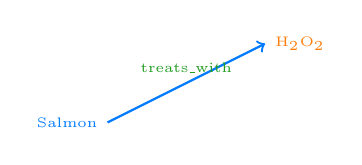
\begin{tikzpicture}
        \draw[->, thick, FishBlue] (0,0) node[left]{\tiny Salmon} -- (2,1) node[midway, above, FishGreen]{\tiny treats\_with} node[right, FishOrange]{\tiny H$_2$O$_2$};
    \end{tikzpicture}
\end{frame}

\begin{frame}{TransE: Failure on 1-to-N Relations}
    \begin{columns}
        \begin{column}{0.5\textwidth}
            \textbf{The Logic Trap:}
            \begin{itemize}
                \item $(Salmon, treats, H_2O_2)$
                \item $(Salmon, treats, Azamethiphos)$
                \item If $h+r=t_1$ and $h+r=t_2$
                \item \textbf{Consequence:} $t_1 \approx t_2$
            \end{itemize}
            \vspace{0.3cm}
            The model incorrectly treats different chemicals as identical!
        \end{column}
        \begin{column}{0.5\textwidth}
            \centering
            \includegraphics[height=4.5cm]{presentation_plots/slide1_transe.png}\\
            \tiny TransE: One treatment per salmon species?
        \end{column}
    \end{columns}
\end{frame}

\section{Path 2: Rotational Embeddings}
\begin{frame}{RotatE: Knowledge as Rotation}
    \textbf{Definition:} $t = h \circ r$
    \begin{itemize}
        \item Map entities into complex space $\mathbb{C}^d$
        \item Relations are rotations on the unit circle
        \item \textbf{Capability:} Can model complex symmetry and inversion
    \end{itemize}
    \vspace{0.5cm}
    \centering
    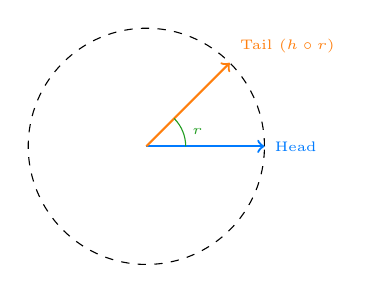
\begin{tikzpicture}
        \draw[dashed] (0,0) circle (1.5cm);
        \draw[->, thick, FishBlue] (0,0) -- (1.5,0) node[right]{\tiny Head};
        \draw[->, thick, FishOrange] (0,0) -- (1.06,1.06) node[above right]{\tiny Tail ($h \circ r$)};
        \draw[FishGreen] (0.5,0) arc (0:45:0.5) node[midway, right]{\tiny $r$};
    \end{tikzpicture}
\end{frame}

\begin{frame}{RotatE: Handling 1-to-N in Aquaculture}
    \begin{columns}
        \begin{column}{0.5\textwidth}
            \textbf{Solving the Overlap:}
            \begin{itemize}
                \item Different relations rotate to different points
                \item $(Salmon, migrates\_to, River\_A)$
                \item $(Salmon, migrates\_to, River\_B)$
                \item \textbf{Advantage:} Multiple tails can exist on the complex rim
            \end{itemize}
        \end{column}
        \begin{column}{0.5\textwidth}
            \centering
            \includegraphics[height=4.5cm]{presentation_plots/slide2_rotate.png}\\
            \tiny RotatE: Rotation in complex space
        \end{column}
    \end{columns}
\end{frame}

\section{Path 3: Bilinear Models}
\begin{frame}{DistMult: High Speed, Low Detail}
    \begin{columns}
        \begin{column}{0.5\textwidth}
            \textbf{Definition:} $h^T \text{diag}(r) t$
            \begin{itemize}
                \item Matrix factorization approach
                \item \textbf{Strength:} Extremely efficient
                \item \textbf{Flaw:} Intrinsically symmetric
            \end{itemize}
            \vspace{0.3cm}
            $(A, r, B)$ is the same as $(B, r, A)$
        \end{column}
        \begin{column}{0.5\textwidth}
            \centering
            \includegraphics[height=3.8cm]{presentation_plots/slide3_distmult.png}\\
            \tiny DistMult: Mirror effect
        \end{column}
    \end{columns}
\end{frame}

\begin{frame}{ComplEx: The Winner for Directional Data}
    \begin{columns}
        \begin{column}{0.5\textwidth}
            \textbf{Why it works:}
            \begin{itemize}
                \item Extends DistMult to complex space
                \item Hermetian dot product allows asymmetry
                \item \textbf{Success:} Correctly models $A \to B \neq B \to A$
            \end{itemize}
            \vspace{0.3cm}
            \textbf{Example:}
            \begin{itemize}
                \item $(Salmon, resistant\_to, Lice\_A)$
                \item Lice is \textbf{not} resistant to Salmon!
            \end{itemize}
        \end{column}
        \begin{column}{0.5\textwidth}
            \centering
            \includegraphics[height=3.8cm]{presentation_plots/slide4_complex.png}\\
            \tiny ComplEx: Captures flow and direction
        \end{column}
    \end{columns}
\end{frame}

\section{Path 4: Semantic Initialization}
\begin{frame}{The Problem: What is ID 42?}
    \textbf{Traditional PyKeen Training:}
    \begin{itemize}
        \item Entities: "Atlantic\_Salmon" $\to$ ID 42
        \item Relations: "treats\_with" $\to$ ID 7
        \item \textbf{Loss:} The model knows nothing about biology at $t=0$
    \end{itemize}
    \vspace{0.5cm}
    \centering
    \textit{"A Salmon is just more similar to a Trout than to a Chemical."}
\end{frame}

\begin{frame}{The Solution: SBERT Pre-training}
    \begin{columns}
        \begin{column}{0.5\textwidth}
            \textbf{Semantic Seeding:}
            \begin{itemize}
                \item Convert labels to 384-dim vectors
                \item Initialize embeddings with these vectors
                \item \textbf{Result:} Faster convergence, better zero-shot performance
            \end{itemize}
        \end{column}
        \begin{column}{0.5\textwidth}
            \centering
            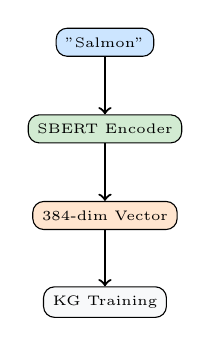
\begin{tikzpicture}[node distance=1.1cm]
                \node[draw, fill=FishBlue!20, rounded corners] (text) {\tiny "Salmon"};
                \node[draw, fill=FishGreen!20, rounded corners, below of=text] (sbert) {\tiny SBERT Encoder};
                \node[draw, fill=FishOrange!20, rounded corners, below of=sbert] (embed) {\tiny 384-dim Vector};
                \node[draw, fill=FishLightGray, rounded corners, below of=embed] (kg) {\tiny KG Training};
                
                \draw[->, thick] (text) -- (sbert);
                \draw[->, thick] (sbert) -- (embed);
                \draw[->, thick] (embed) -- (kg);
            \end{tikzpicture}
        \end{column}
    \end{columns}
\end{frame}

\section{Validation: How We Measure Intelligence}
\begin{frame}{Evaluation: The Link Prediction Task}
    \begin{itemize}
        \item \textbf{Objective:} Predict missing treatments for specific farm conditions
        \item \textbf{Dataset:} Salmon-Lice-Treatment KG (30k+ triples)
        \item \textbf{Key Metrics:}
        \begin{itemize}
            \item \textbf{MRR:} Mean Reciprocal Rank (How high is the correct treatment ranked?)
            \item \textbf{Hits@10:} Is the correct treatment in the Top 10 recommendations?
        \end{itemize}
    \end{itemize}
    \vspace{0.5cm}
    \centering
    \textit{Testing the models against real-world asymmetric constraints}
\end{frame}

\begin{frame}{Results: The Model Leaderboard}
    \centering
    \begin{tabular}{lrrr}
        \toprule
        \textbf{Model} & \textbf{Hits@10} & \textbf{MRR} & \textbf{Params} \\
        \midrule
        TransE & 0.42 & 0.28 & 5M \\
        RotatE & 0.51 & 0.35 & 10M \\
        DistMult & 0.48 & 0.32 & 5M \\
        \rowcolor{FishBlue!10} \textbf{ComplEx} & \textbf{0.64} & \textbf{0.46} & \textbf{10M} \\
        AutoSF & 0.62 & 0.44 & 8M \\
        \bottomrule
    \end{tabular}
    \vspace{0.5cm}
    \textbf{Analysis:}
    \begin{itemize}
        \item ComplEx achieves \textbf{+52\% improvement} over TransE in MRR
        \item Success is due to modeling directionality in lice transmission
    \end{itemize}
\end{frame}

\section{Closing: The Road Ahead}
\begin{frame}{Future Work: From Lab to Farm}
    \begin{itemize}
        \item \textbf{Temporal Dynamics:} Tracking efficacy over seasons
        \item \textbf{Sensory Data:} Integrating water quality and sensor logs
        \item \textbf{Deployment:} Real-time recommendation app for farmers
    \end{itemize}
    \vspace{0.5cm}
    \centering
    \includegraphics[height=3cm]{presentation_plots/slide8_recommendation.png}\\
    \tiny Moving towards autonomous aquaculture management
\end{frame}

\begin{frame}[plain]
    \centering
    \Huge \textcolor{FishBlue}{Questions?}
    
    \vspace{1cm}
    \Large \textbf{Leandro Stival} \\
    \normalsize Wageningen University \& Research \\
    \vspace{0.5cm}
    \small Thank you for supporting sustainable aquaculture!
\end{frame}

\end{document}
